%!TeX root=../tese.tex
%("dica" para o editor de texto: este arquivo é parte de um documento maior)
% para saber mais: https://tex.stackexchange.com/q/78101

%% ------------------------------------------------------------------------- %%

% "\chapter" cria um capítulo com número e o coloca no sumário; "\chapter*"
% cria um capítulo sem número e não o coloca no sumário. A introdução não
% deve ser numerada, mas deve aparecer no sumário. Por conta disso, este
% modelo define o comando "\unnumberedchapter".
\chapter{Duckietown}
\label{cap:duckietown}

%% ------------------------------------------------------------------------- %%
\section{O que é Duckietown?}
\label{sec:o-que-e-duckietown}

\enlargethispage{.5\baselineskip}

Duckietown\index{Duckietown} é um modelo de ensino de inteligência artificial com foco em veículos autônomos. Esse modelo, cujo desenvolvimento se deu em 2016 pelo MIT\index{MIT} para ser usado na disciplina de mesmo nome, é uma simplificação do tráfego urbano de veículos e serve de porta de entrada para as áreas da robótica e da automação~\citep{duckietown-historia}. Apesar de tudo isso o Duckietown é bem robusto, como pode ser visto na figura~\ref{fig:duckietown_exemplo}, ao contar com ruas de mãos duplas, intersecções, calçadas, obstáculos e pedestres além de ser flexível para permitir o aumento gradual da complexidade do problema e a criação de inúmeros cenários a serem estudados e resolvidos.

\begin{figure}
	\centering
	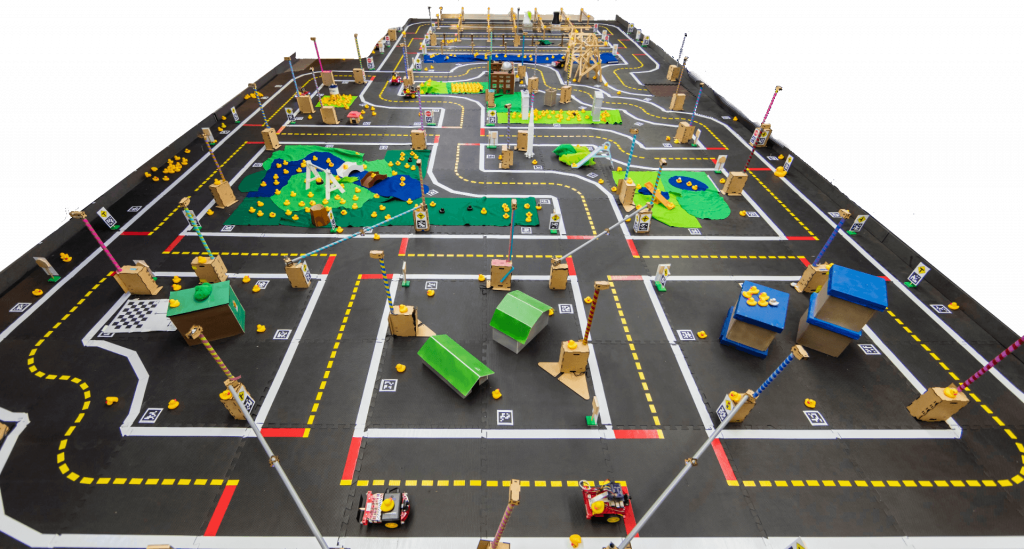
\includegraphics[width=.8\textwidth]{duckietown_exemplo}
	\caption{Exemplo de Duckietown (figura retidade de~\citep{duckietown-guia}).\label{fig:duckietown_exemplo}}
\end{figure}

Ademais, o desenvolvimento do Duckietown teve como um dos principais objetivos que ele fosse acessível com o intuito de que o modelo viesse a ser utilizado por instituições de ensino de todo o planeta. O veículo ou, como batizado, Duckiebot foi projetado para não só ser a plataforma mais simples e barata com a qual é possível se ensinar uma disciplina avançada de autonomia, como também, é completamente open source. Logo, nos anos seguintes o Duckietown se expandiu rapidamente e em 2018 foi fundada a \emph{Duckietown Foundation}, uma organização sem fins lucrativos, com a missão de tornar a robótica e inteligência artificial acessíveis e inclusivas pelo mundo. 

\section{Gym-Duckietown}

Este trabalho utiliza o simulador\index{simulador} Gym-Duckietown\citep{gym-duckietown}\index{Gym-Duckietown} para o treino e execução do veículo autônomo. Esse simulador do universo de Duckietown teve seu início em 2018, dentro do ecossistema Gym desenvolvido pela OpenAI\index{OpenAI}\citep{1606.01540}, como parte do trabalho feito pelo \textit{Mila - Quebec AI Institute} e com o passar do tempo o projeto evoluiu para um simulador de direção autônoma completamente funcional, que pode ser usado para treinar e testar sistemas de aprendizado de máquina, além dos algoritmos clássicos da robótica como árvores de decisão ou veículos de \textit{Braitenberg}. Por último, o Gym-Duckietown possui diversas ferramentas para recriar complicações reais, como distorção de câmera, além de aleatorização de domínio para evitar o \textit{overfit} do modelo ao simulador.

\begin{figure}
	\centering
	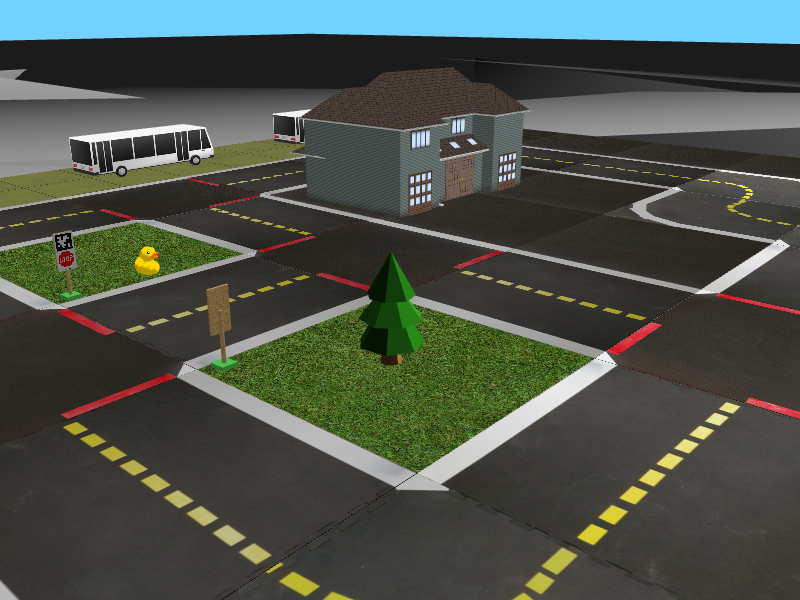
\includegraphics[width=.8\textwidth]{simulador_exemplo}
	\caption{Imagem do Gym Duckietown (imagem retidade de~\citep{gym-duckietown}).\label{fig:simulador_exemplo}}
\end{figure}


